\documentclass[a4paper]{report}
\renewcommand{\chaptername}{}
\usepackage{graphicx}


\begin{document}
%cover page

\titlepage 
\begin{center}
\LARGE\textbf{MagPY}\\[.5cm]
\large\textit{MAIN PROJECT REPORT}\\[0.5cm]
\textit{submitted in partial fulfillment of the requirements for the award of the degree of}\\[.5cm]
\textnormal{Bachelor of Technology}\\[0.5cm]
\textnormal{in}\\[.5cm]
\large \textbf {COMPUTER SCIENCE AND ENGINEERING}\\[.5cm]
\textnormal{of}\\[.5cm]
\large \textbf {MAHATMA GANDHI UNIVERSITY}\\[.5cm]
\textnormal{by}\\[.5cm]
\large \bfseries{








PAUL JACOB V(11012351)\newline
SARATH S MENON(11012367)\newline
THUMSSY P NAZAR(11012380)\newline













}

\vspace{0.25cm}
\includegraphics[width=3.0cm]{logo.png}\\[0.5cm]
\vspace{.25cm}
\textnormal{Department of Computer Science and Engineering}\\[0.5cm]
\textnormal{Rajagiri School of Engineering and Technology}\\[0.5cm]
\textnormal{Rajagiri Valley, Kakkanad, Kochi, 682039}\\[0.5cm]
\textnormal{2015}\\[0.5cm]
\end{center}

\newpage
\begin{center}
\fontsize{17.28pt}{19.2pt}
\textbf{ACKNOWLEDGEMENT}\\[1.0cm]
\end{center}
\pagenumbering{roman}
\setcounter{page}{2}
\addcontentsline{toc}{chapter}{Acknowledgement}
\vspace{1.0cm}
\paragraph{}
\large\textnormal{A special gratitude to our final year project guide, Mr. Jayarajan J. N, Assistant Professor ,whose contribution in stimulating suggestions and encouragement, helped us to coordinate our project especially in writing this report. He has assisted us through the entire project by providing the required modifications in each stage and evaluating continuously so that we could attain our target in right time.}

\paragraph{}
\large\textnormal{ We also thank our lab in-charge Ms. Mary Priya Sebastian,Assistant Professor, for her guidance and provided us with all support inside our lab. We thank our Mini Project in-charge Mrs. Gopika S, Assistant Professor, for giving timely instructions during the entire journey of our project. We have to appreciate the guidance given by other supervisor as well as the panels especially in our project presentation that has improved our presentation skills thanks to their suggestions and advices. We also thank other lab in-charge teachers namely Fr. Jaison Paul Mulerickal, Assistant Professor and Dr. John Jose, Assistant Professor too. I also thank the head of the institution Dr. A. Unnikrishnan ,Principal and the head of the department Mr.Ajith S, Assistant Professor for all your support and co-operation.}

\paragraph{}
\large\textnormal{The entire project was made possible by providing us with the required machines and software’s by our college lab staffs, we thank them too. Furthermore we would also like to acknowledge our college and department of computer science for all their support and providing us with the required facilities.}

\newpage
\begin{center}
\fontsize{17.28pt}{19.2pt}
\textbf{ABSTRACT}\\[1.0cm]
\end{center}
\pagenumbering{roman}
\setcounter{page}{3}
\addcontentsline{toc}{chapter}{Abstract}
\vspace{1.0cm}
\paragraph{}
\large\textnormal{MagPY is a constraint based web document extractor,developed based on web scraping and web crawling.The Magpy is a project aimed at bringing about a better web search experience by providing a constraint based search rather than the simple keyword based approach as done by popular search engines like Google, Yahoo and Bing. The constraints are of different type,including negation of some words, size limit for the result, repetitions, regular expressions etc.Also, with a system to watch a web page for certain updates and with the ability to provide data from just targeted section of the page, MagPY improves the speed, accuracy and reduces the burden of the user to a large extent. }
\paragraph{}
\large\textnormal{In brief, this project is focused on producing a web based document extraction tool presented in a simple GUI, and provides the capabilities to search using keywords and regular expressions, and along with it, constrain the results based on different criteria. It acts as an advancement over the modern search engines by providing the capability to filter results and partial load web pages for contents or peek into the web pages, which is not possible in the current scenario.}
\paragraph{}
\large\textnormal{Taking into consideration the working of present search engines and crawlers, they work on the basis of the metadata like description, tags, SEO tips and keywords that are provided by the website creator. This can be a disadvantage if “keyword stuffing” or similar technique is used to fool the search engine, and be on top of their results. But MagPy does the job of further drilling down into the page and filtering the real and fake pages out.This project has got application in various domains like research, data mining, marketing etc. This project is going to be developed in Python and will run on platforms like Windows and Android.}

\newpage
\pagenumbering{arabic}
\setcounter{page}{1}
%\begin{spacing}{}
%\label{sec:Problem statement}
\chapter{Introduction}
\paragraph
\large\textnormal{Current web search experience experiences a lot of drawbacks including the
inability to use constraints in the search results, like to negate a keyword, limit the size of results, or to provide only results having a specified size, target only specific region of the result page rather than loading the whole page for viewing just a small portion of it and so on.With this project, we aim at removing all these limitations and provide a much better, simple, efficient, fast and fluidic experience in web search.}

\large\textnormal{MagPy is a constraint based web document extractor, a project aimed at bringing about a better web search experience by providing a constraint based search rather than the simple keyword based approach as done by popular search engines like Google, Yahoo and Bing. The constraints are of different type, including negation of some words, size limit for the result, repetitions, regular expressions
etc. Also, with a system to watch a webpage for certain updates and with the ability to provide data from just targeted section of the page, MagPy improves the speed, accuracy and reduces the burden of the user to a large extent.}
\paragraph{}
\large\textnormal{In brief, this project is focused on producing a web based document extraction tool presented in a simple GUI, and provides the capabilities to search using keywords and regular expressions, and along with it, constrain the results based on different criteria. It acts as an advancement over the modern search engines by providing the capability to filter results and partial load web pages for contents or peek into the web pages, which is not possible in the current scenario.}
\paragraph{}
\large\textnormal{This project involves an application front-end that needs to be simple and user friendly, as well as support all major platforms available. This is an important constraint due to the number of platforms that are present now.Another constraint is a good internet connection, as scrapping web data involves large amount of data to be transferred, in a short time. But since most of the load of getting data from various websites and processing it is taken by the server, to the user, network usage would not be much of a limitation. Additionally, because of the inbuilt partial-load feature, data usage would be minimal in the long run.We are based on APIs provided by search engines like Google, Yahoo and Bing, So interfacing those APIs would be the next, but a minor design issue.Next issue is the storage requirement on the server side. Multiple user requests involve a large amount of websites to be scrapped, and a lot of data in involved in its processing.}
\paragraph{}
\large\textnormal{This project utilizes data obtained from a large number of web sources, and hence has large dependencies. But since the initial step of selecting the top data sources is done by top and advanced search engines like Google and Yahoo, the possibility of erroneous sources is reduced, and we can safely assume that the data obtained is authentic, irrespective of the sources and the queries.Another important dependency arises due to the use of APIs provided by various providers, though they won’t bring out sudden, unnoticed changes, there should be a watch on the limitations and updates done to the APIs in the long run. However, we have planned a system that would make the system comparatively immune to API changes, thus reducing effects on the actual system.}

\paragraph{}
\large\textnormal{Along with these functionalities, MagPy also provides a bunch of other constraints that
are not present in the current system, or are not easy to implement. With top results extracted from top search engines like Google, Bing and Yahoo, the results provided by MagPy are comparatively more efficient than the results provided by any search engine alone. Another case is that where the user needs to search for contents semantically, as the example of kingfisher. The user can simply specify a negation of the term airlines to imply that what the user needs is not about kingfisher airlines, but about the bird.}

\paragraph{}
\large\textnormal{Taking into consideration the working of present search engines and crawlers, they work
on the basis of the metadata like description, tags, SEO tips and keywords that are provided by the website creator. This can be a disadvantage if “keyword stuffing” or similar technique is used to fool the search engine, and be on top of their results. But MagPy does the job of further drilling down into the page and filtering the real and fake pages out.This project has got application in various domains like research, data mining, marketing etc. This project is going to be developed in Python and will run on platforms like Windows and Android.}

\chapter{Literature Survey}

\chapter{Hardware and Software Specifications}
There are no major external components involved in the development of this project. The components of the software itself are only the server and the client apps, which are clearly explained earlier.
The hardware and software requirements for the user to use the final 
product are as follows:
Hardware:
PC users:

Minimum 1 gigahertz (GHz) or faster 32-bit (x86) or 64-bit (x64) processor 256 MB of RAM

Mobile Users:

Minimum 800 Megahertz (MHz) or faster processor 100 MB of RAM

Software:
PC Users:
Python pre-installed

Mobile Users:
None.

\chapter{System Analysis and Design}

Our project makes use of the Object Oriented Analysis and Design approach of development. This helps in modelling the various components of the project Object-oriented analysis and design (OOAD) is a popular technical approach to analyzing, designing an application, system, or business by applying the object-oriented paradigm and visual modeling throughout the development life cycles to foster better stakeholder communication and product quality. It imitates the real world entities very easily.The purpose of any analysis activity in the software life-cycle is to create a model of the system's functional requirements that is independent of implementation constraints.During object-oriented design (OOD), a developer applies 
implementation constraints to the conceptual model produced in object-oriented analysis. Such constraints could include the hardware and software platforms, the performance requirements, persistent storage and transaction, usability of the system, and limitations imposed by budgets and time.Object-oriented modeling (OOM) is a common approach to modeling applications, systems, and business domains by using the object-oriented paradigm throughout the entire development life cycles. OOM is a main technique heavily used by both OOA and OOD activities in modern software engineering.
\section{Data Design}
\begin{center}

\begin{figure}
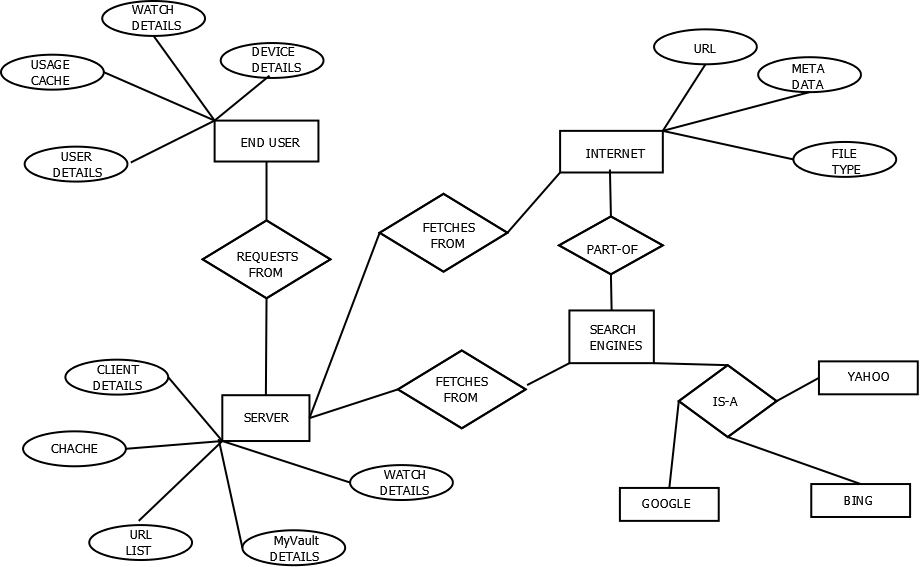
\includegraphics[width=10.0cm]{MagPy_Entity.png} 
\end{figure}

\end{center}

\paragraph{}
\large\textnormal{The Entities and their relationships are indicated with their attributes in the diagram. The advantage of using object based approach can be highlighted in this, as most of the components are correlated and represented easily than compared to how it would be, in a functional model.}

\paragraph{}
\large\textnormal{This project does not involve any hardware interfacing requirements, as the final product is a software that can be accessed as an app of a web service, irrespective of the device.In terms of the design language, the user interface that we are targeting is based on the modern trend called the card based design. This approach is being used by most leading firms including Google.}

\large\textnormal{\newline\newline1.	The transmitted signal bandwidth is much greater than the information bandwidth.\newline
2.	Some function other than the information being transmitted is employed to determine the resultant transmitted bandwidth.
}
\begin{center}
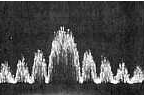
\includegraphics[width=5.0cm]{dsss.png}\\[0.75cm]
\end{center}
\begin{center}
\small\textnormal{Figure 1.2.1:A Spectrum Analyzer Photo of a Direct Sequence (DS) Spread Spectrum signal} 
\end{center}
\paragraph{}
\large\textnormal{Most commercial part 15.247 spread spectrum systems transmit an RF signal bandwidth as wide as 20 to 254 times the bandwidth of the information being sent. Some spread spectrum systems have employed RF bandwidths 1000 times their information bandwidth. Common spread spectrum systems are of the "direct sequence" or "frequency hopping" type, or else some combination of these two types (called a "hybrid").}
\begin{center}
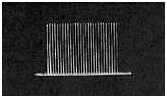
\includegraphics[width=5.0cm]{fhss.png}\\[0.75cm]
\end{center}
\begin{center}
\small\textnormal{Figure 1.2.2:A Spectrum Analyzer Photo of a Frequency Hop (FH) Spread Spectrum signal }
\end{center}
\paragraph{}
\large\textnormal{There are also "Time Hopped" and "Chirp" systems in existence. Time hopped spread spectrum systems have found no commercial application to date. However, the arrival of cheap random access memory (RAM) and fast micro-controller chips make time hopping a viable alternative spread spectrum technique for the future. "Chirp" signals are often employed in radar systems and only rarely used in commercial spread spectrum systems.}

\subsection{ Direct Sequence Systems}
\large\textnormal{Direct sequence spread spectrum systems are so called because they employ a high speed code sequence, along with the basic information being sent, to modulate their RF carrier. The high speed code sequence is used directly to modulate the carrier, thereby directly setting the transmitted RF bandwidth. Binary code sequences as short as 11 bits or as long as [2\^(89) - 1] have been employed for this purpose, at code rates from under a bit per second to several hundred megabits per second.}
\paragraph{}
\large\textnormal{The result of modulating an RF carrier with such a code sequence is to produce a signal centered at the carrier frequency, direct sequence modulated spread spectrum with a (sin x/x)2 frequency spectrum. The main lobe of this spectrum has a bandwidth twice the clock rate of the modulating code, from null to null. The sidelobes have a null to null bandwidth equal to the code's clock rate. Figure 1 illustrates the most common type of direct sequence modulated spread spectrum signal. Direct sequence spectra vary somewhat in spectral shape depending upon the actual carrier and data modulation used. The signal illustrated is that for a binary phase shift keyed (BPSK) signal, which is the most common modulation signal type used in direct sequence systems.}

\subsection{ Frequency Hopping Systems}
\large\textnormal{The wideband frequency spectrum desired is generated in a different manner in a frequency hopping system. It does just what its name implies. That is, it "hops" from frequency to frequency over a wide band. The specific order in which frequencies are occupied is a function of a code sequence, and the rate of hopping from one frequency to another is a function of the information rate. The transmitted spectrum of a frequency hopping signal is quite different from that of a direct sequence system. Instead of a [(sin x)/x]\^2-shaped envelope, the frequency hopper's output is flat over the band of frequencies used. Figure  shows an output spectrum of a frequency hopping system. The bandwidth of a frequency hopping signal is simply w times the number of frequency slots available, where w is the bandwidth of each hop channel.}
\section{What Spread Spectrum Does}
\paragraph{The use of these special pseudo noise codes in spread spectrum (SS) communications makes signals appear wide band and noise-like. It is this very characteristic that makes SS signals possess the quality of Low Probability of Intercept. SS signals are hard to detect on narrow band equipment because the signal's energy is spread over a bandwidth of maybe 100 times the information bandwidth.}
\paragraph{}
\large\textnormal{The spread of energy over a wide band, or lower spectral power density, makes SS signals less likely to interfere with narrowband communications. Narrow band communications, conversely, cause little to no interference to SS systems because the correlation receiver effectively integrates over a very wide bandwidth to recover an SS signal. The correlator then "spreads" out a narrow band interferer over the receiver's total detection bandwidth. Since the total integrated signal density or SNR at the correlator's input determines whether there will be interference or not. All SS systems have a threshold or tolerance level of interference beyond which useful communication ceases. This tolerance or threshold is related to the SS processing gain. Processing gain is essentially the ratio of the RF bandwidth to the information bandwidth.}
\paragraph{}
\large\textnormal{A typical commercial direct sequence radio, might have a processing gain of from 11 to 16 dB, depending on data rate. It can tolerate total jammer power levels of from 0 to 5 dB stronger than the desired signal. Yes, the system can work at negative SNR in the RF bandwidth. Because of the processing gain of the receiver's correlator, the system functions at positive SNR on the baseband data.}
\paragraph{}
\large\textnormal{Besides being hard to intercept and jam, spread spectrum signals are hard to exploit or spoof. Signal exploitation is the ability of an enemy (or a non-network member) to listen in to a network and use information from the network without being a valid network member or participant. Spoofing is the act of falsely or maliciously introducing misleading or false traffic or messages to a network. SS signals also are naturally more secure than narrowband radio communications. Thus SS signals can be made to have any degree of message privacy that is desired. Messages can also, be cryptographically encoded to any level of secrecy desired. The very nature of SS allows military or intelligence levels of privacy and security to be had with minimal complexity. While these characteristics may not be very important to everyday business and LAN (local area network) needs, these features are important to understand.}

\chapter{PN sequences}
\paragraph{}
\large\textnormal{A pseudo random noise (PN) sequence is a sequence of binary numbers. Eg:-+1 or -1 which appears to be random; but is in fact perfectly deterministic. The sequence appears to be random in the sense that the binary values and groups or runs of the same binary value occur in the sequence in the same proportion they would if the sequence were being generated based on a fair coin tossing experiment. In the experiment each head could result in one binary value and a tail the other value. The PN sequences appears to have been generated from such an experiment. The software or hardware used to produce PN sequence is called a PN generator}
\paragraph{}
\large\textnormal{A PN sequence generator is typically N cascaded flip flops circuits and a specially selected feedback arrangement. The flip flops used in this way is called a shift register since each clock pulse applied to the flip flops causes the contents of each flip flop to be shifted to the right. The feedback connections provide the input to the left most flip flop. With N binary stages, the largest number of different patterns the shift register can have is 2N. However, the all zero binary state is not allowed because it would cause all remaining states of the shift register and its outputs to be binary zero. The all binary ones state does not cause a similar problem of repeated binary ones provided the number of flip flops input to the module 2 adder is even. The period of the PN sequence is therefore 2N-1.}
\paragraph{}
\large\textnormal{A PN sequence has three following properties:}\\
\textnormal{1. The number of ‘1’s and the number of ‘0’s in a PN sequence are only different by one.}\newline\newline
\textnormal{2. Run lengths of zeroes or ones are the same as in a coin flipping experiment. Half of the run lengths are unity, one-quarter are of length two, one-eighth are of  length three and a fraction 1/2n  of all runs are of length n.}\newline\newline
\textnormal{3. If the sequence is shifted by any non-zero number of elements, the resulting sequence will have an equal number of agreements and disagreements with the original sequence.}\\
\section{Applications of PN sequences}
\textnormal{1.PN sequences widely uses in CDMA communication system. It can acquire in the presence of channel error, false detection can be minimized without reducing the frame efficiency by using a long sequence multiplexed with the data.}\newline\newline
\textnormal{2. PN sequence uses in Spread spectrum modulation to spread the RF bandwidth of the signal, reducing the power spectral density.}\newline\newline
\textnormal{3.  PN sequence also use for scrambling the data at the same rate to obtain spectral energy distribution within the signal band.}\\
\chapter{Linear Feedback Shift Register(LFSR)}
\paragraph{}
\large\textnormal{LFSR is used to generate the simplest PN sequences.It is a shift register whose input is a linear function of previous state.The linear function of single bits is exclusive or.The initial value is called seed.Operation of the register is deterministic ,hence the stream of values produced is completely determined by the previous or current state.After a finite number of possible states, it enters the repeating cycle.
Using a well defined feedback ,Random sequence can be obtained.}
\section{Maximal length sequences}
\paragraph{}
\large\textnormal{Maximal length sequences are the largest codes that can be generated using linear feedback shift register. The PN sequences is like a high noise frequency signal, binary in nature thus it look like pulses. It is not a completely random but it is generated by a well defined logic. The same logic is used at the transmitter and receiver. The pseudo noise sequences can be generated by a feedback shift register and the combinational logic. The data of one shift register is shifted to the next one whenever a clock pulse is applied. The output of the shift registers is given to the logic circuit depending on the output of the shift registers the output of the logic circuit  is decided. This logic circuit is given as the input to the first shift register. The PN sequence is generated at the output of the last shift register. At each clock pulse, the state of the shift register to next shift register and the logic circuit in the first shift register. The PN sequence generated at the output shift register is repeated after 2m   digits which is also called as the period of the PN sequence. Normally the logic circuit used is the mod 2 adders. If the shift register enters the zero state it will not come out of it and output sequence will be only zeros. To prevent this problem, zero state of the shift register is not allowed. Therefore the total number of states in the m feedback shift register is 2m-1, therefore the output pseudo noise sequence will also have a period of 2m-1.   When the PN sequence generated by LFSR has the length of 2m -1, it is called the maximal length sequence.}
\begin{center}

\end{center}
\begin{center}
\small\textnormal{Figure 3.1.1:m sequence generator for a polynomial}
\end{center}
\chapter{30 percent of the main project}
\section{Program in Matlab }
\large\textnormal{s=[1 0 1 0];\\
t =[4 3];\\
n=length(s);\\
c(1,:)=s;\\
m=length(t);\\
for k=1:2$^n$-2;\\
b(1)=xor(s(t(1)),s(t(2)));\\
if m$>2;\\
    for i=1:$m-2;\\
    b(i$+1)=xor(s(t(i$+2)), b(i));\\
    end\\
end\\
j=1:n$-1;\\
s(n$+1$-j)=s(n$-j);\\
s(1)=b(m$-1);\\
c(k$+1,:)=s;\\
end\\
seq=c(:,n);}
\section{Program in Xilinx}
\large\textnormal{module mkrs1(o,clk,rst);\\
parameter lng=4;\\
parameter inistate=4'b1001;\\
parameter[1:lng] tapco=4'b0011;\\
input clk,rst;\\
output o;\\
reg o;\\
reg[1:lng] y;\\
reg x;\\
always @(posedgeclk)\\
if(~rst)\\
begin\\
y=inistate;\\
o=y[4];\\
end\\
else\\
begin\\
x=y[4];\\
y[4]=y[3];\\
y[3]=y[2];\\
y[2]=y[1];\\
y[1]=y[4] xor x;\\
o=y[4];\\
end\\
endmodule}


\begin{center}
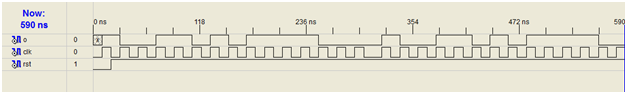
\includegraphics[width=15.0cm]{lfsro.png}\\[0.75cm]
\end{center}
\begin{center}
\small\textnormal{Figure 4.2:Output of FPGA implementation of LFSR}
\end{center}













\end{document}
\end